\begin{wrapfigure}[0]{r}[9pt]{0cm}
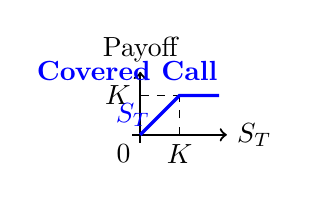
\begin{tikzpicture}[scale=1]
    % --- 定义坐标和参数 ---
    \def\K{0.5}       % 执行价格 K
    \def\maxST{1}     % S_T 的最大显示范围

    % --- 绘制坐标轴 ---
    % X 轴 (S_T)
    \draw[->, thick] (-0.1, 0) -- (\maxST + 0.1, 0) node[right] {$S_T$};
    % Y 轴 (Payoff)
    \draw[->, thick] (0, -0.1) -- (0, \K + 0.3) node[above] {Payoff};

    % --- 绘制辅助线和标签 ---
    % 在 x 轴上标记 K
    \draw[dashed, thin] (\K, 0) node[below] {$K$} -- (\K, \K);
    % 在 y 轴上标记 K (最大收益水平)
    \draw[dashed, thin] (0, \K) node[left] {$K$} -- (\K, \K);
    % 标记原点
    \node[below left] at (0,0) {0};

    % --- 绘制组成部分 (灰色虚线) ---
    % 1. Long Underlying Asset (Payoff = S_T)
    % 通过原点，斜率为 1 的直线
    %\draw[gray, dashed, thick] (0, 0) -- (\maxST, \maxST);


    % 2. Short K-strike Call Option (Payoff = -max(S_T - K, 0))
    % 在 S_T < K 时为 0，在 S_T > K 时斜率为 -1
    %\draw[gray, dashed, thick] (0, 0) -- (\K, 0) -- (\maxST, \K - \maxST);


    % --- 绘制最终的 Covered Call Payoff (蓝色粗线) ---
    % Covered Call Payoff = Long Asset + Short Call = S_T - max(S_T - K, 0)
    % 当 S_T <= K 时，Payoff = S_T - 0 = S_T (斜线)
    % 当 S_T > K 时，Payoff = S_T - (S_T - K) = K (水平线)
    \draw[blue, very thick] (0, 0) -- (\K, \K) -- (\maxST, \K);

    % --- 添加简化的标签 ---
    % 斜线段的 Payoff = S_T
    \node[blue, left] at (\K/2, \K/2) {$S_T$};
    % 水平段的 Payoff = K
    % 总标签
    \node[blue, anchor=south east, font=\bfseries,xshift=3pt,yshift=2pt] at (\maxST, \K) {\textbf{Covered Call}};

\end{tikzpicture}
\end{wrapfigure}